\documentclass{ifacconf}

\usepackage{graphicx}      % include this line if your document contains figures
\usepackage{natbib}        % required for bibliography

\def\Section {\S}
%===============================================================================
\begin{document}
\begin{frontmatter}
%\title{ Decentralized Multi-robot Control\\ Using HEAD: Hybrid Event-driven Architecture on D-Bus   \thanksref{footnoteinfo}} 
%\title{ Flexible Multi-robot Control\\ Using HEAD: Hybrid Event-driven Architecture on D-Bus   \thanksref{footnoteinfo}} 
% Title, preferably not more than 10 words.
\title{Flexible Communication in Multi-robotic Control System Using HEAD: Hybrid Event-driven Architecture on~D-Bus   \thanksref{footnoteinfo}} 

\thanks[footnoteinfo]{This research has been funded by the Engineering and Physical Sciences Research Council (EPSRC), UK, grant reference EP/E061915/1.}

\author{Md Omar Faruque Sarker and } 
\author{Torbj{\o}rn S. Dahl.} 

\address{Robotic Intelligence Lab, University of Wales, Newport\\
Allt-yr-yn Campus, Allt-yr-yn Avenue, Newport, NP205DA, UK\\
 (e-mail: Mdomarfaruque.Sarker|Torbjorn.Dahl@newport.ac.uk)}

\begin{abstract}                % Abstract of not more than 250 words.
Direct real-time communication among various software components of a multi-robot system (MRS) is much more complicated than that in software simulations. Existing inter-process communication (IPC) mechanisms, such as pipes, shared memory etc., are very rigid and usually enforce tight coupling among software components. Thus they do not integrate well with heterogeneous multi-robot control applications of a relatively larger MRS that typically consists of tens of robots and various sensing and monitoring elements interconnected through several host PCs. In this paper, we present a modular, flexible and decentralized multi-robot control architecture, namely hybrid event-driven architecture on D-Bus (HEAD), that overcomes these issues by decoupling IPC through D-Bus. D-Bus is a relatively newer IPC technology for modern Linux desktop environments. It typically uses a message bus daemon that facilitates asynchronous data sharing among multiple processes. Here, we show that by using only a single type of message, namely D-Bus {\em signal} type, HEAD can efficiently enable real-time interactions among heterogeneous multi-robot control applications. The design of HEAD is flexible enough to add various types of existing and new software components with minimum programming effort. As an example, we present how we achieve a decentralized peer-to-peer communication behaviours among robot controller clients by simply adding only a few lines of new code leaving the major IPC implementation intact. This paper also reports the performance of D-Bus, under both constant and variable IPC load, obtained from our MRS implementation of a manufacturing shop-floor scenario with 16 e-puck robots.
\end{abstract}

\begin{keyword}
multi-robot system, real-time control, inter-process communication, D-Bus
%Five to ten keywords, preferably chosen from the IFAC keyword list.
\end{keyword}

\end{frontmatter}
%===============================================================================
\section{Introduction}
Inter-process communications (IPC) among various desktop software components enable them to talk to each other and exchange data, messages or request of services. Technological advancements in computer and communication systems  now allow robotic researchers to set-up and conduct experiments on multi-robot systems (MRS) from  desktop PCs. Many compelling reasons, including open licensing model, availability of open-source tools for almost free of cost, community support etc., make Linux as the most preferable operating system for MRS research. However the integration of heterogeneous software components in Linux desktop becomes a challenging issue, particularly when each robot-control software (hereafter called robot-controller client or RCC for short) needs sensory and other data input from various other software components (e.g. pose data from a tracker server, task information from a task server etc.).  
Traditional IPC solutions in a standard Linux desktop, e.g. pipes, sockets, X atoms, shared memory, temporary files etc. (hereafter called {\em traditional IPCs}),  are too heterogeneous to meet the demand of a dynamic software system \cite{Wittenburg2005}. On the other hand, complex and heavy IPC like CORBA fails to integrate into a development tool-chain efficiently. They also require a steep learning curve due to their complex implementations. Besides, the failure of Desktop Communication Protocol (DCOP) in system-wide integration and interoperability encouraged the development  of the D-Bus message bus system (D-Bus for short).

D-BUS was designed from scratch to replace CORBA and DCOP and to fulfil the needs of a modern Linux system. D-BUS can perform basic application IPC, allowing one process to shuttle data to another. D-BUS can facilitate sending events, or signals, through the system, allowing different components in the system to communicate and ultimately to integrate better. D-BUS is unique from other IPC mechanisms in several ways, e.g. 1) the basic unit of IPC in D-BUS is a message, not a byte stream, 2) D-BUS is bus-based and 3) It has separate system-wide and user/session-wide bus  \cite{Love2006} . The simplest form of communication is process to process. D-BUS, however, provides a daemon, known as the message bus daemon, that routes messages between processes on a specific bus. In this fashion, a bus topology is formed, allowing processes to speak to one or more applications at the same time. Applications can send to or listen for various events on the bus.

%===============================================================================
\section{D-Bus Communication Model}
%%%%%%%%%%%%%%%%%%
\subsection{D-Bus Overview}
\begin{figure}
\begin{center}
\includegraphics[width=7cm,height=3.1cm]{./dia-files/dbus-daemon}    % The printed column width is 8.4 cm.
\caption{A typical view of D-Bus message bus system } 
\label{fig:abstract-arch}
\end{center}
\end{figure}


%%%%%%%%%%%%%%%%%%
\subsection{Strategies for Application Integration}

%===============================================================================
\section{Hybrid Event-driven Architecture on D-Bus (HEAD)}
%%%%%%%%%%%%%%%%%%
\subsection{Overview of Multi-robot Control}
\begin{figure}
\begin{center}
\includegraphics[width=2.5cm,height=2.1cm]{./dia-files/three-layer-arch}    % The printed column width is 8.4 cm.
\caption{Classical three layer robot control architecture \cite{Gat1997}} 
\label{fig:abstract-arch}
\end{center}
\end{figure}
%% 
\begin{figure}
\begin{center}
\includegraphics[width=5.5cm,height=2.1cm]{./dia-files/abstract-arch}    % The printed column width is 8.4 cm.
\caption{Our abstract multi-robot control architecture} 
\label{fig:abstract-arch}
\end{center}
\end{figure}
%%%%%%%%%%%%%%%%%%
\subsection{Characteristics of {\em HEAD}}
\subsection{D-Bus Overview}
\begin{figure*}
\begin{center}
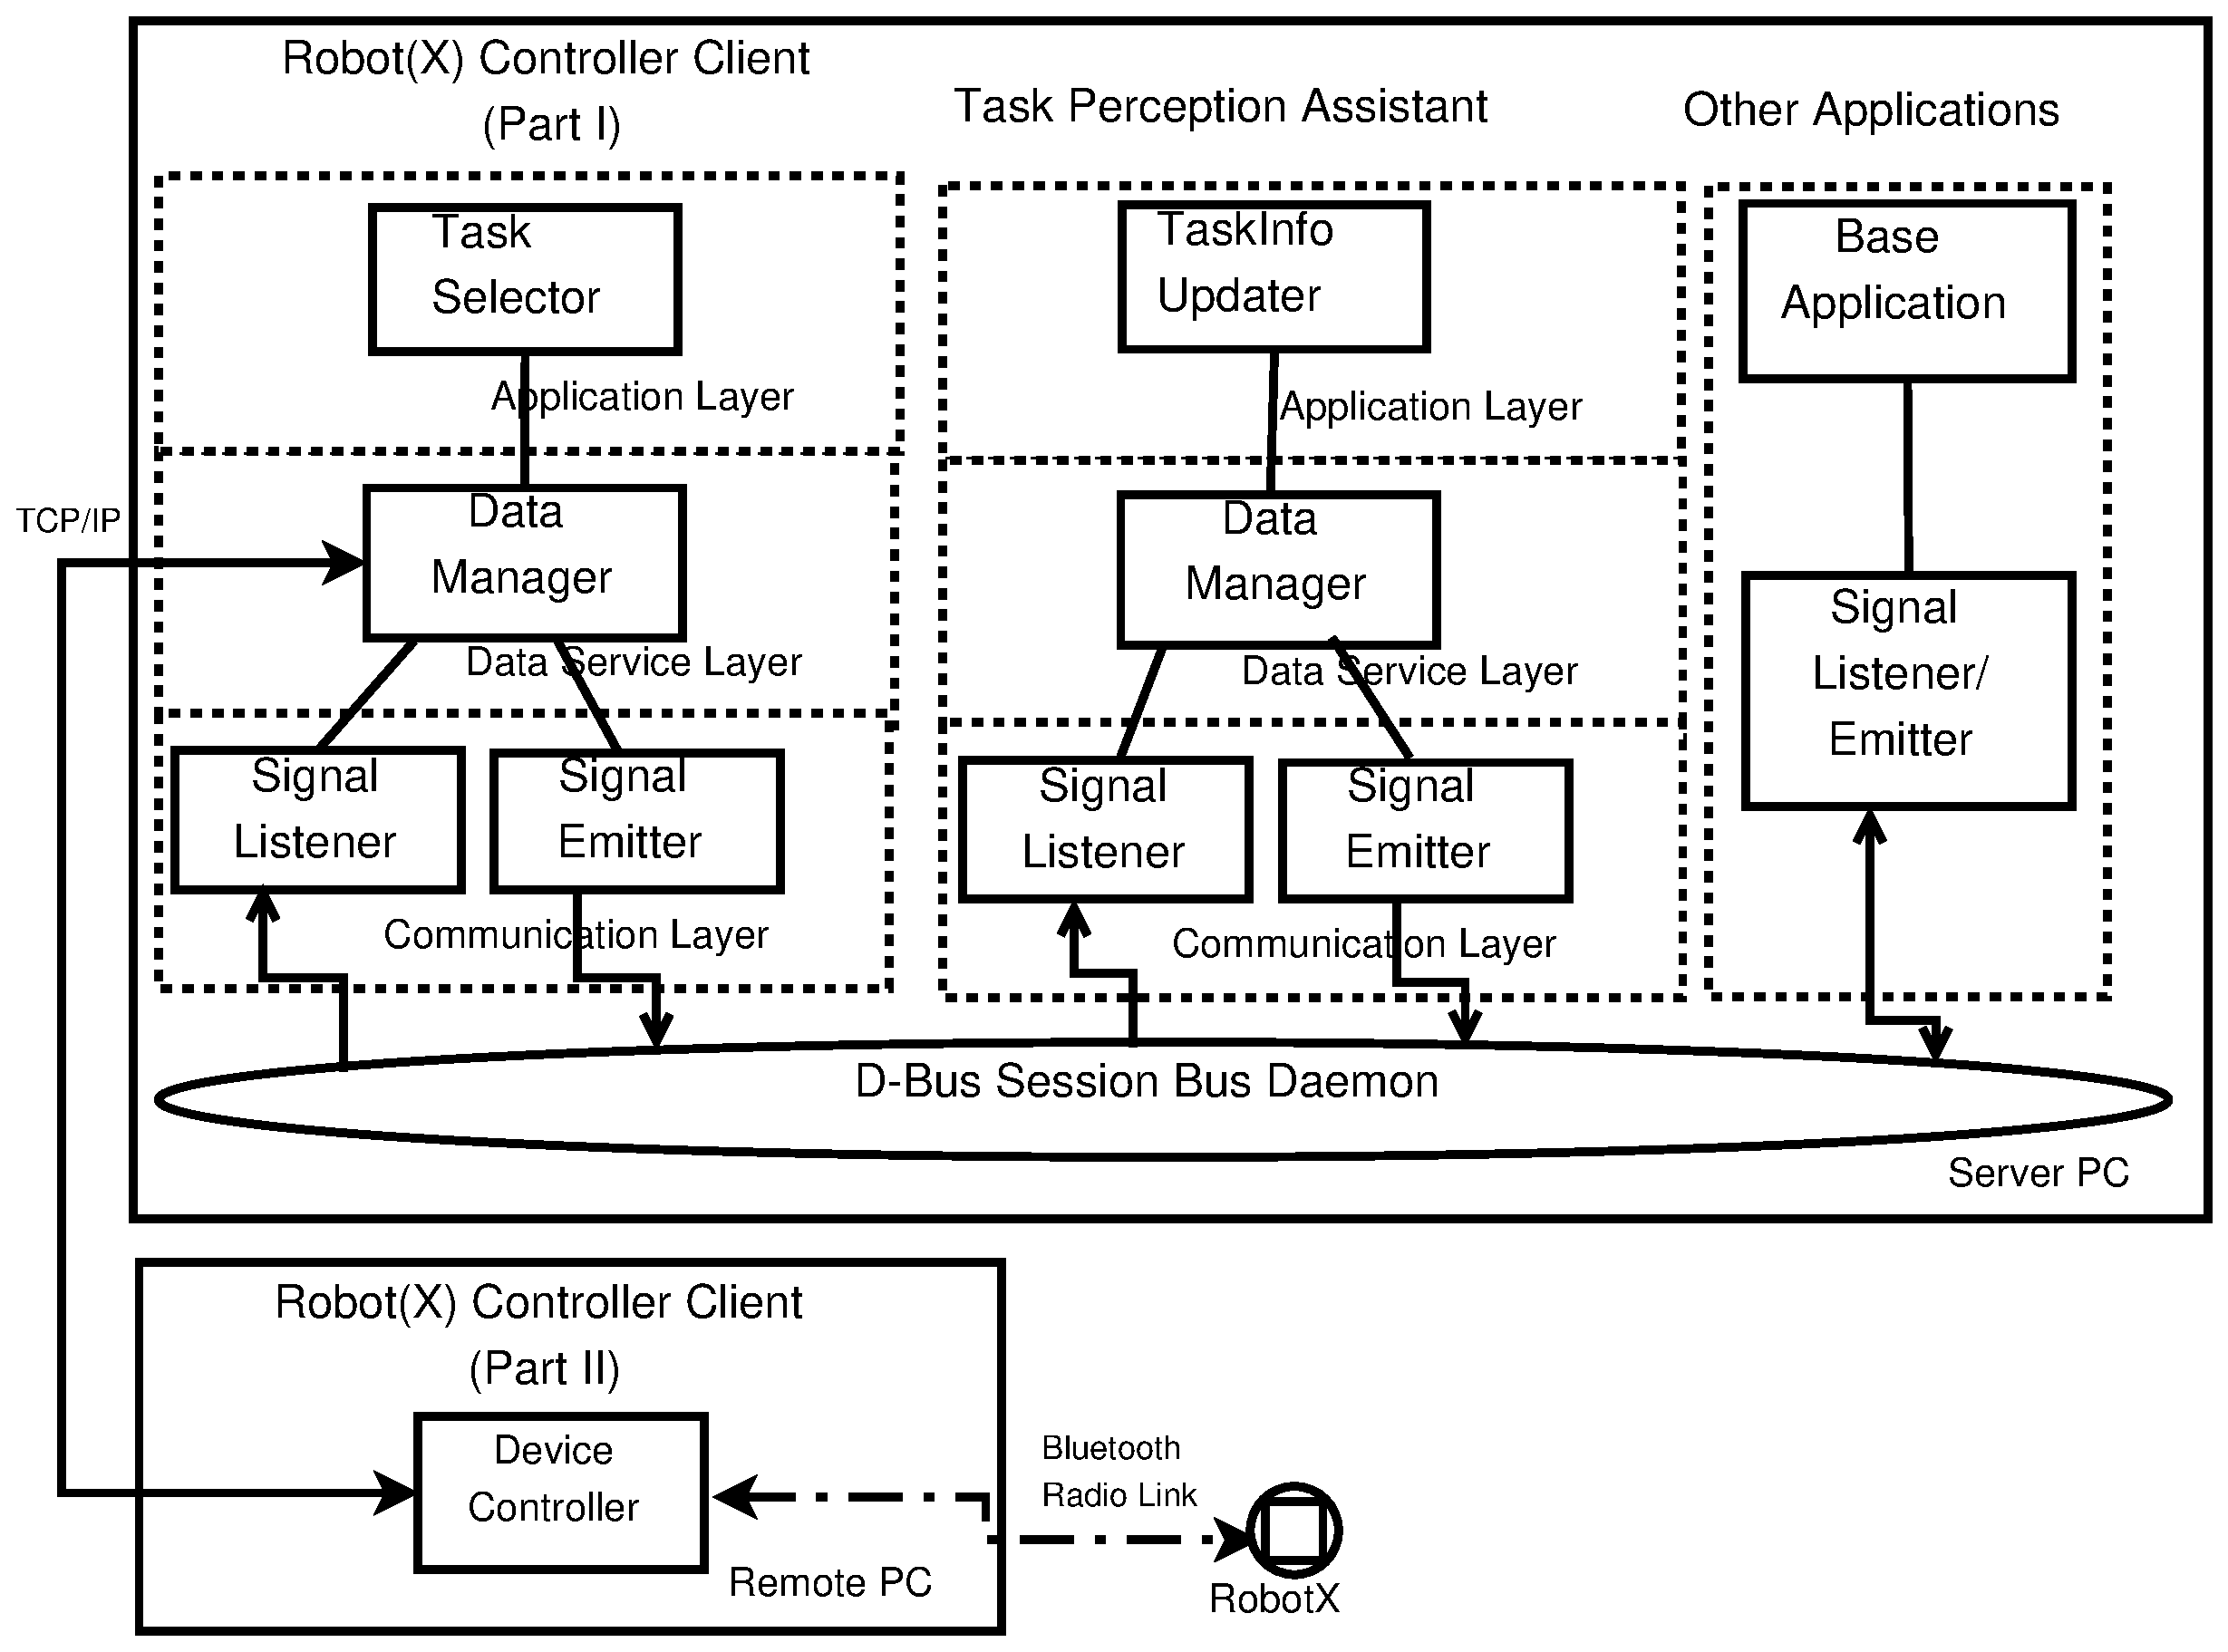
\includegraphics[width=12cm,height=8cm]{./dia-files/concrete-arch}    % The printed column width is 8.4 cm.
%\centering
\caption{General outline of {\em HEAD}. Robot-Controller-Client application has been splitted into two parts: one runs locally in server PC and another runs remotely, e.g., in embedded PC} 
\label{fig:abstract-arch}
\end{center}
\end{figure*}


%%%%%%%%%%%%%%%%%%
\subsection{D-Bus Signal Interfaces}

%%%%%%%%%%%%%%%%%%
\subsection{Common Interfaces}
%	D-Bus Signal Listener
% 	D-Bus Signal Emitter


%%%%%%%%%%%%%%%%%%
\subsection{Integration of Software Components}

%===============================================================================
\section{Flexible Communication  Schemes of {\em HEAD}}
%%%%%%%%%%%%%%%%%%
\subsection{Centralized Communication}

%%%%%%%%%%%%%%%%%%%
\subsection{Decentralized Communication}


%===============================================================================
\section{Implementation of a Multi-robot Manufacturing Scenario}
\subsection{Characteristics of {\em HEAD}}
\subsection{D-Bus Overview}
\begin{figure*}
\begin{center}
\includegraphics[width=12cm,height=8cm]{./dia-files/RIL-Expt-Setup3}    % The printed column width is 8.4 cm.
%\centering
\caption{An example implementation of {\em HEAD}. Robot-Controller-Clients can talk to each other and exchange task information through D-Bus signals} 
\label{fig:abstract-arch}
\end{center}
\end{figure*}

%%%%%%%%%%%%%%%%%%%%%%%%%%%%%%%%%%%%%%%%
\subsection{Multi-robot Task Allocation}
%% 
\begin{figure}
\begin{center}
\includegraphics[width=7.5cm,height=5cm]{./images/PlotUrgencyLog-2010Feb15-171017}    % The printed column width is 8.4 cm.
\caption{Dynamic changes in task urgencies} 
\label{fig:task-urgency}
\end{center}
\end{figure}

%%%%%%%%%%%%%%%%%%%%%%%%%%%%
\subsection{Experiment Setup}


%%%%%%%%%%%%%%%%%%%%%%%%%%%%%%%%%%%
\subsection{Results and Discussions}
%% 
\begin{figure}
\begin{center}
\includegraphics[width=7.5cm,height=5cm]{./images/Global-SignalingFreqStat}    % The printed column width is 8.4 cm.
\caption{D-Bus task information signalling frequency of TPA in centralized communication mode} 
\label{fig:global-freq}
\end{center}
\end{figure}
%% 
\begin{figure}
\begin{center}
%\includegraphics[width=7.5cm,height=5cm]{./images/Robot12-16feb-1-LocalSignals}     
\includegraphics[width=7.5cm,height=5cm]{./images/Robot12-17feb-3-LocalSignals}
\caption{Robot12's simultaneous reception of task information signals from peers} 
\label{fig:robot-freq}
\end{center}
\end{figure}
%%
\begin{figure}
\begin{center}
\includegraphics[width=7.5cm,height=5cm]{./images/Local-500cm-SignalingFreqStat}    % The printed column width is 8.4 cm.
\caption{Local P2P task information signalling frequency of all robots in decentralized communication mode} 
\label{fig:global-freq}
\end{center}
\end{figure}



%===============================================================================
\section{Conclusion}

%A conclusion section is not required. Although a conclusion may review the main points of the paper, do not replicate the abstract as the conclusion. A conclusion might elaborate on the importance of the work or suggest applications and extensions.

%\begin{ack}
%Place acknowledgments here.
%\end{ack}

\bibliography{control2010}             % bib file to produce the bibliography
                                                     % with bibtex (preferred)
                                                   
\appendix
\section{D-Bus Listener Code}    % Each appendix must have a short title.

\section{D-Bus Emitter Code}              % Sections and subsections are supported  
                                                                         % in the appendices.
\end{document}